\section{Information and Communication Technologies in Developing Countries}

It is important to take notice of what kind of development \gls{ict}'s are supposed to support.
And in this notion make conclusions and measures based on that.
Like increase a countries competitiveness in the global free market.
Common problems that concerns the \gls{is} in developing countries are:

\begin{itemize}
\item Scarce resourses
\item Little technology
\item Missing skills
\end{itemize}

\subsection{Discourses}
\label{subsec:discourses}
\begin{itemize}
\item The pace and direction is set by the advanced economies in the world, North America and Europe. \cite{ca:isdc}
\item An increasing number of studies in developing countries in Africa, Asia and Latin America.
\item Developing countries are highlighting new topics like national culture, global politics, provision of \gls{ict} resources for a community.
\item 
\end{itemize}
\begin{description}
\item[\textit{Transfer and Diffusion Discourse}]
	The Transfer and Diffusion discourse assumes that \gls{is}-innovations in developing countries are achieved by transferring technology and organizational structure from more advanced countries. Much like, "if it works here, it should work there". In order to succeed the receiving part should try to emulate what is being done in the more developed countries. Of course \gls{is} these ideas of best practice are somewhat adapted to fit their new context, but the underlying assumption is that the transferred methods result in the same outcomes.
\item[\textit{Social Embeddednes Discourse}]
	This discourse assumes that \gls{is} innovation is about creating new techno-organizational structures given a local social context. The new structures are built on the already existing structures and are a locally socially constructed course of action. The problems are seen from a local perspective and hence the solutions has to be an integrated part.
\item[\textit{Transformative Discourse}]
	The last discourse is mostly concerned with creating possibilities for improvement of life conditions. It focuses on how \gls{is} can be used to facilitate deep socio-economic change.
	The social embeddednes discourse takes the local context into consideration, but the transformative takes it one step further and includes politics, economics and social conditions. 
\end{description}

The transformative discourse raises more explicitly the strategic issues in the development struggle.

A distinctive feature of \gls{is} research in developing countries is that it puts focus on e-governments, free and open software and the development of community resources intended to overcome the digital divide.

Issues that received attention in \gls{isdc}.
\begin{itemize}
\item \gls{is}-failure
\item Outsourcing
\item The strategic role of \gls{ict}
\end{itemize}

Diffusion and transformative development does not facilitate the already existing structures of the context the technology will be placed within.
The implementation of information systems from this perspective requires the environment and the people in it to adapt to the new technology.
This will in turn increase the risk of the information system being rejected by the users. On the other hand, the socially embedded path
will to some extent safeguard the underlying social structures by building upon what is already there. 
This might lead to unexpected results and be time consuming. Although, probably avoiding the sustainability pitfall.

\cite{ca:isdc}

\subsection{Success and Failure of ISDC}
\label{successandfailure}

Are there any evidence suggesting that there are more \gls{is}-failures in developing countries?




In the \gls{isdc} literature the is an anxiety about failure, and not without reason.
Compared to other settings there are additional pressures.
The need to catch up with the rest of the world, high opportunity costs and over optimistic expectations.




Categories of failure:
\begin{itemize}
\item Scalability failure because of waning political support, technological complexity, human resource capacity.
\item Sustainability failure because of starvation of \gls{is} resource, loose political commitment, poorly maintained. This could be tracked down to foreign aid-donors that neglected the development of local technological capabilities. The remedy is of course to look at \gls{is} as the socially embedded instead of transfer and diffusion. The \gls{is} project needs to be an integrated part of organizational practices, secure the required financial and knowledge based resources and political commitment in order to succeed.
\item Assimilation in dysfunctional organizational processes, meaning that an already broken system cannot be fixed with facilitating the broken system with \gls{is}.
\end{itemize}





\begin{description}
\item[Total Failure] An initiative that never is implemented or abandoned immediately after implementation.
\item[Partial Failure] An initiative where major goals are unattained or where there are significant undesirable outcomes.
\item[Success] An initiative where major goals are attained for most stakeholders and there are no significant undesirable outcomes.
\end{description}




\begin{figure}
\centering
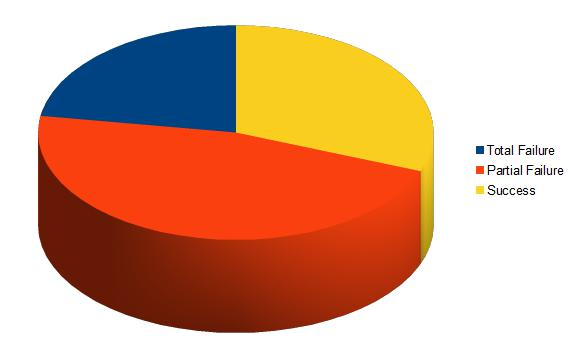
\includegraphics[width=\textwidth]{literature/img/failChart}
\caption{Diagram of Success and Failures in Industrialized Countries}
\label{fig:failchart}
\end{figure}

In industrialized countries there is an estimate of $\frac{12}{60}$ to $\frac{15}{60}$ fall into the category of total failure; something like $\frac{20}{60}$ to $\frac{36}{60}$ fall in the partial failure category; and lastly the $\frac{9}{60}$ to $\frac{28}{60}$ are successes. See figure \ref{fig:failchart}.

For practical reasons like lack of technical and human infrastructure developing countries should be performing worse than industrialized countries.
The evidence base is not that strong due to lack of literature in general, evaluation and focus on case studies, but it generally points in one direction. High rates of \gls{is}-failure.

Failure can be viewed as something positive. 
Like in a learning process, but it cannot be overlooked that continually failing keeps the under developed countries on the wrong side of the digital divide. 

Organizational change can be viewed as a process between two states.
The current system and the future.
The future system would represent the design of a \gls{is} system that are to be implemented.
And the current system as a description of how the system is.
Between these models there will need to be some change in several dimensions like processes, people, structure and technology in order to reach the a state of the future system. This design-actuality gap usually represents how much risk are involved from moving to a design. 

The actuality of the industialized countries and developing countries have in themselves gaps.
The design-actuality gap might not be the same for the solutions used in industrialized countries and developing countries. 

\cite{rh:isdc}
\cite{ca:isdc}







\section{Outsourcing}
Offshoring has it's spring from:

\begin{itemize}
\item globalization of trade in services
\item Software commoditization
\item Wage differentials
\item Business friendly climate 
\item Growth of offshore labor pool
\item Drop in telecom costs
\end{itemize}

China graduates four times more engineers than the \gls{usa} pr. year. 
Before there were a differance in the quality of the engineering program, but the gap has narrowed. 
The talent was always there, but before those with talent would emigrate to industrialized countries. 
With globalization of trade in services we can tap into their services from anywhere. 
With low telecom prizes, low wages and software commoditization industrialized countries are able to offshore their software activities more or less. 

The wage factor are the most dominant factor for off-shoring.
The global software work phenomenon is not the first of it's kind, but it differs in that it delivers a service rather than a specific product. 
It is well known that manufactoring and production are often moved to other low-wage countries.
Parts of software development has now become such a commodity that firms from industrialized countries are able to outsource these tasks and keep the more high-level activity for themselves. 

A useful way of understanding this context is via Vernon's \textit{international product cycle}.
\begin{description}
\item[\textit{Stage 1:}]\hfill
A new product begin with highly skilled entrepreneural activities, typically in industrialized nations.
\item[\textit{Stage 2:}]\hfill
Production begin to shift offshore via investments in low-wage nations.
\item[\textit{Stage 3:}]\hfill
As the product standardizes, it is mass produced with cheap, low-skilled labor.
\end{description}


Software has areas in all three stages. The high-level activities stay in stage 1 while being prepared as routine tasks of best practice, then moved towards stage 3 through stage 2.

Global Software Work opens up a market that are very different from others.
The developing countries are here able compete under very different circumstances.
Were the developed countries has to deal with high salaries the developing countries can benefit from having lower salaries and compete on cost. This makes the market highly dependent on the knowledge competencies. As discussed in section \ref{infolearnec} a countries ability to learn has a great impact for developing the economy. Access to knowledge intuitively has a way of speeding up the learning process. And the most efficient way of getting to knowledge is through \gls{ict}'s. 
Having the opportunity to compete on knowledge competencies can pace the way for developing countries. By focusing on learning the developing countries of the world are able to enter the market of \gls{ict}'s with an advantage. Policy makers in charge of economic growth and infrastructure should therefore recognize this and facilitate both the learning process and the exportation of services. 
By focusing on this area of expertise development in other areas of industry are likely.
Having a highly developed \gls{ict} infrastructure is likely to have spillover effects on the domestic services and production. Making opportunities for even new innovations. 
History has shown that there is a link between fortunes of the developed countries and the developing. Rapid upgrades in \gls{ict}'s have reduced the costs and increased the scope of operations all over the world. 

A number of developing countries have nurtured software and \gls{ict} services industries able to compete in the global market, India being the most successful. 
Factors that account for success in the global market include technology and project management skills, copyright legislation and government industrial policy. By making an effort to outsource, there may be also be an increase to services offered to the domestic organizations. This in turn will have an impact on the overall developments of the country or region. It is hard to imagine that there are little technological use in a place that are among the top exporters of software. The spill over effect may results in local organizations running better, and this way offering better possibilities in the other fields as well.

\cite{ca:isdc}
\cite{sbs:gio}
\cite{offit:paan}




\section{Digital Divide}

\section{ICT4D}
Giving attention to \gls{ict}'s in the developing countries are both rewarding and useful. 
The potential impact \gls{ict}'s have in developing countries are much greater than in the industrialized countries. 
An innovative \gls{ict}'s step in the industrialized countries may lead to some improvemnt in productivity, but focusing our efforts in the developing countries has the potential of a much bigger impact.
The world problems of conflict, desease and resource depletion are first met by the poor. 
Although the more advanced economies of the world are not primary victims, it is beneficial to give these problems some attention.
These problems may someday reach the industrialized countries someday through terror, desease epedemics and migration. 
There is also the case that if the poor get richer, they buy more products. 


In the 21st century economic, social and political life are increasingly becoming more digital. 
This is also the case for the developng countries. An estimate from 2012 shows that  $34.3\%$ of the global population has internet access.
The computers entered the developing countries in 1954, Kolkata India.
Initially computing was used in the developng countries in the public sectors for adminastrive tasks, but in the 1980's some saw \gls{ict}'s potential for economic growth in the private sectior.
With the internet really catching on in the 1990's, giving much attention to \gls{ict}'s and the political focusing on the international development, gave rise to \gls{ict4d}
Initially computing was used in the developng countries in the public sectors for adminastrive tasks, but in the 1980's some saw \gls{ict}'s potential for economic growth in the private sectior.
The internet really grew during the the 1990's, giving much attention to \gls{ict}'s.
At the same time international development was moving up on the political agenda.
Combines these two subjects gave rise the the concept of \gls{ict4d}.
As a result, initiatives like telecenter was taken place.
These were buildings housing computers giving people access to the world wide web.
The initiative had some problems succeeding, but brought with them important lessons that are still challenges we are facing today.
Sustainability, scalability and evaluation of systems in the developing countries are important topics to consider.
The systems of the past had a tendency to fail to deliver, have a limited reach and was generally talked about as better outcomes than it in reality was.

The main goal of the future should be to give internet access to the remaining $65.7\%$ of the population.
With this goal in mind there are two ways to go. Either lean on existing technologies or wait for the technological innovations.
Here it is possible to go both ways. 

Introducing \gls{ict}'s can done in three different ways.
One could just set up an environment and make the users adapt to existing processes, work with the users and continually innovate making locally appropriate solutions or lastly just introduce the technology and have the users innovate on their own. 

\cite{internet:stats}
\cite{icd4d:rh}


\begin{quotation}
Lack of literature in general: Until very recently,
the entire literature on IS and developing countries
would struggle to ll a single bookshelf. The
attention of writers—from researchers to consultants
to journalists—has been focused elsewhere.\cite{rh:isdc}
\end{quotation}
\begin{quotation}
Lack of evaluation: Those who have the will to
evaluate—such as academics—often lack the
resources and capacity. Those who have the
resources—such as aid donor agencies—often
lack the will to evaluate.\cite{rh:isdc}
\end{quotation}
\begin{quotation}
Focus on case studies: The literature on IS in
DCs has grown, but it is a literature dominated by
case studies of individual IS projects. Taken alone,
these provide no basis for estimation of overall
failure/success rates.\cite{rh:isdc}
\end{quotation}

\section{Pitfalls in introducing IS in Developing Countries}
\subsection{Scalability}
The problem of moving expertise and system to new locations with the lessons learned.
By conceptualize the use of ICT's one can make it easier to transfer ICT's to other locations, making it scalable.\cite{jbemss:noa}.
\subsection{Sustainability}
What happens when the AID funded projects stops being funded? The donors are interested in sustainable solutions that keep existing after the investment.
How does one maintain a project that is built on temporary donors. Unfortunately many IS projects are drained from resources \cite{ca:isdc}.
Here should it be mentioned something about political commitment \cite{jbemss:noa}.  

\subsection{Assimilation In Dysfunctional Organizational Processes}
One has to take into account that an already broken system can't be fixed by speeding it up.
Automating a process that already does not produce the right result would only give us more of the result we are trying to change \cite{mh:rw}.









\subsection{Lack of persistence on key areas}







\section{Evidence base}

\begin{quotation}
Health information systems in South Africa: Braa
and Hedberg (2002) reported widespread partial
failure of high cost systems with little use of data.\cite{rh:isdc}
\end{quotation}

\begin{quotation}
IS in the Thai public sector: Kitiyadisai (2000)
reported “failure cases seem to be the norm in
Thailand at all governmental levels.”\cite{rh:isdc}
\end{quotation}

\begin{quotation}
Donor-funded IT projects in China: Baark and
Heeks (1999) reported that all were found to be
partial failures.\cite{rh:isdc}
\end{quotation}

\begin{quotation}
World Bank-funded IT projects in Africa: Moussa
and Schware (1992) reported almost all as partial—
often sustainability—failures.\cite{rh:isdc}
\end{quotation}

\section{Untapped Marked}
From a certain perspective one can see the developing countries as an untapped marked.
By building up the countries infrastructure one has the opportunity to offer services that previously was not possible.
Take Telenor and their agenda to offer insurance and banking services in the east.
By building up the infrastructure they can now offer their services as "mobile providers" and even expand their services to banking with a fresh market and less competition.


\section{Sustainability}
\cite{jbemss:noa}

Building networks running on the same concept will make the ICT initiative more sustainable. 

User participation is another tool one can use in order to make ICT initiative more sustainable.
When the concept is accepted and made by the users they understand how and why it works and are more likely to accept it.
